\documentclass[nochapterpage,bigchapter,linedtoc,longdoc,colorback,accentcolor=tud1c]{tudreport}
\usepackage{ngerman}

\usepackage[stable]{footmisc}
\usepackage[ngerman]{hyperref}

\usepackage{longtable}
\usepackage{multirow}
\usepackage{booktabs}

\hypersetup{%
  pdftitle={Entwicklung und Test einer
eingebetteten Elektronik für einen
innovativen Schaltaktor},
  pdfauthor={Malte Breitenbach, Johannes Faupel, Jonas Tautz, Johanna Vetter},
  pdfsubject={Beispieltext},
  pdfview=FitH,
  pdfstartview=FitV
}

%%% Zum Tester der Marginalien %%%
  \newif\ifTUDmargin\TUDmarginfalse
  %%% Wird der Folgende Zeile einkommentiert,
  %%% werden Marginalien gesetzt.
  % \TUDmargintrue
  \ifTUDmargin\makeatletter
    \TUD@setmarginpar{2}
  \makeatother\fi
%%% ENDE: Zum Tester der Marginalien %%%

\newlength{\longtablewidth}
\setlength{\longtablewidth}{0.7\linewidth}
\addtolength{\longtablewidth}{-\marginparsep}
\addtolength{\longtablewidth}{-\marginparwidth}


% \settitlepicture{tudreport-pic}
% \printpicturesize

\title{Entwicklung und Test einer eingebetteten Elektronik für einen innovativen Schaltaktor}
\subtitle{Malte Breitenbach, Johannes Faupel, Jonas Tautz, Johanna Vetter}
%\subsubtitle{email: \textaccent{tud-design@pro-kevin.de}}
%\setinstitutionlogo[width]{TUD_sublogo}
%\uppertitleback{(\textaccent{\textbackslash uppertitleback})}
\lowertitleback{\hfill\today}
\institution{ 
Institut für Mechatronische Systeme im Maschinenbau\\
     Prof. Dr.-Ing. Stephan Rinderknecht}
%\dedication{Hier ist gen"ugend Platz\\
  %f"ur eine Widmung (\textaccent{\textbackslash dedication}).\\
  %\strut\\
  %F"ur Annelore Schmidt\\
  %aus dem Referat Kommunikation.\\
  %Sie hat immer ein offenes Ohr\\
  %f"ur unsere Fragen und Anregungen.}
%\sponsor{\color{tud9b}\rule{\linewidth}{7mm}}
%\sponsor{\hfill\includegraphics[height=6ex]{tud_logo}\hspace{1em}
\includegraphics[height=6ex]{TUD_chaos}}

\begin{document}
\maketitle
\begin{abstract}
Hier könnte Ihr Abstract stehen.
\end{abstract}  

\tableofcontents

%% Hier Tex-Dateien includen
%%%%%%%%%%%%%%%%%%%%%%%%%%%%%%%%%%%%%%%%%%
\chapter{Einleitung}
\section{Motivation}


\section{Ziele der Arbeit}
Auch das Institut für Mechatronische Systeme (IMS) der TU Darmstadt nimmt sich dieser Aufgabe an und arbeitet im Rahmen des Projektes Speed4E, dass einen elektrifizierten Antriebsstrang mit Peak-Antriebsdrehzahlen von bis zu $50.000/min$ zum Ziel hat, an einem innovativem Schaltaktor. Im Verlauf vorheriger Arbeiten wurde bereits ein Tauchspulenaktor ausgelegt sowie eine Elektronik für ihn entwickelt. Das Ziel dieser Arbeit ist es nun, die bisherigen Funktionen auf einen Mikrocontroller zu implementieren sowie eine eingebettete Elektronik zu entwerfen, die den Aktor zu einem Smart Actuator transformiert. Des Weiteren sollen Sicherheits- und Überwachungsfunktionen für den Aktor entwickelt werden und Statusmeldungen per CAN gesendet werden. 

\section{Anforderungsliste}
Um das übergeordnete Ziel weiter zu spezifizieren wurde zunächst  eine Anforderungsliste erstellt. In dieser sind alle Forderungen an das Endprodukt gesammelt, sie dient damit als Basis und Referenz für die Produktentwicklung. Die Liste ist hierbei dynamisch, das heißt sie kann im Verlauf des Entwicklungsprozesses verändert oder ergänzt werden.  Die formulierten Anforderungen werden schließlich noch nach Priorität kategorisiert und einer der vier folgenden Anforderungsarten (Quelle: Pahl (2004): Konstruktionslehre - Grundlagen erfolgreicher Produktentwicklung - Methoden und Anwendung S. 189.) zugeteilt:
Festforderungen (FF) sind unter allen Umständen einzuhalten. Eine Erfüllung ist für eine erfolgreiche Lösung notwendig.
Bereichsforderungen (BF) geben einen Toleranzbereich an, innerhalb dessen sich der schlussendlich erreichte Wert befinden muss.
Zielforderungen (ZF) geben an, welcher Wert (auch im Hinsicht auf spätere Entwicklungen) angestrebt wird.
Wünsche (W) sollten nach Möglichkeit erfüllt werden, sind aber keine Voraussetzung. 

\begin{table}[h]
	\centering
		\begin{tabular}{l|p{7cm}|p{7cm}}
			\textbf{Relevanz} & \textbf{Anforderung} & \textbf{Erläuterung} \\ \hline
			& &\\
			FF & Benutzerfreundliche Kommunikation durch CAN Schnittstelle & Empfang von Befehlen, Senden von Statusmeldungen \\
			FF & Nichtflüchtige Kalibrierung & Eine Kalibrierung ist nur einmalig und zur Rekalibrierung notwendig \\
			BF & Schaltzeit & < 100 ms (Latenz zwischen Senden des Befehls und vollständig ausgeführtem Gangwechsel) \\
			FF & Selbstständige Fehlererkennung & Überstrom, Temperatur, Eingangsspannung (OVP/UVP), Dekalibrierung \\
			FF & Schnittstellen & CAN, 8-12VDC Versorgung (max XA), Programmierschnittstelle (für Updates \& Bugfixes) \\
			W & Wartbarkeit & Sicherung wechseln im eingebauten Zustand \\
			BF & kompakte Baugröße & \\ 
			BF & Effizienz (gemittelt über einen Schaltvorgang) & elektrischer Wirkungsgrad > 90 \% \\
			FF & Temperaturbeständigkeit & bis 105°C \\
			BF & Aktorüberschwingen & Toleriert, solange kein unbeabsichtigter Gangwechsel \\
			W & Schaltgabelkraft am Anschlag & möglichst gering \\
			FF & Standby & Standbyleistungsaufnahme < 5W \\
		\end{tabular}
	\caption{Anforderungsliste}
	\label{tab:Anforderungsliste}
\end{table}

\section{Vorgehen der Arbeit}
Nachdem in der oben stehenden Anforderungsliste die Ziele der vorliegenden Arbeit definiert wurden, soll nun das weitere Vorgehen zum Erreichen der Zielsetzung erläutert werden. Zunächst werden in Kapitel 2 der Stand des Prüfstands vor Beginn des ADPs sowie wichtige Grundlagen als Basis für die weitere Bearbeitung und zum besseren Verständnis dargelegt. In Kapitel 3 werden die verschiedenen Bauteile, die für die eingebettete Elektronik benötigt werden, und ihre Funktionen beschrieben. Außerdem wird der erste Prototyp und sein Entwicklungsprozess beschrieben. Kapitel 4 beschäftigt sich mit der Implementierung der Funktionalität in Matlab Simulink BLABLABLA
In Kapitel 5 soll schließlich das endgültige Platinendesign vorgestellt werden.
\chapter{Prüfstand}
\section{Grundlagen des Prüfstandes}
In diesem Kapitel wird der verwendete Schaltaktorikprüfstand des IMS vorgestellt, an dem  die Entwicklung des Smart Actuators stattgefunden hat. Die Konstruktion des Prüfstandes erfolgte in vorangegangenen Arbeiten und wurde seitdem stetig weiterentwickelt. An ihm werden Schaltaktoriksysteme für Fahrzeugantriebe untersucht. Abbildung \ref{fig:Pruefstand} zeigt die in dieser Arbeit verwendeten Subsysteme des Prüfstandes. Im Folgenden erfolgt zunächst die Vorstellung des mechanischen Aufbaus, woraufhin der elektronische Aufbau anschließt. 

\begin{figure}[h]
	\centering
<<<<<<< HEAD
		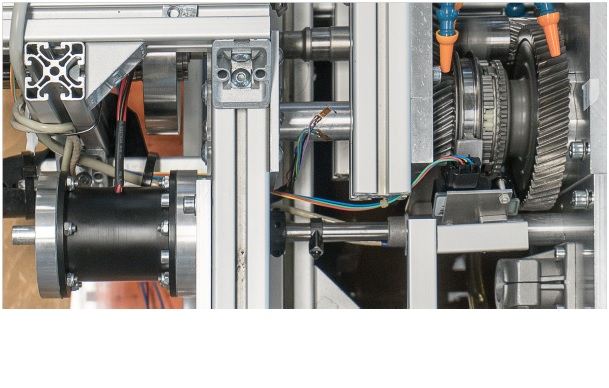
\includegraphics{Bilder/Pruefstand.jpg}
=======
	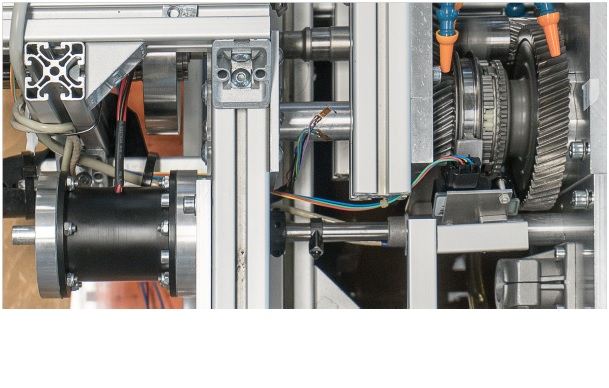
\includegraphics{./Bilder/Pruefstand.jpg}
>>>>>>> cc7043c638d4a861f6d73a6ccf59b0ffca8d4bdd
	\caption{Prüfstand}
	\label{fig:Pruefstand}
\end{figure}

\subsection{Getriebe allgemein}

Ein Getriebe ist im Automobil dafür zuständig, die Drehzahl des Motors in ein Drehmoment umzuwandeln, welches die Räder antreibt. Da Motoren nur einen kleinen Bereich von Motordrehzahlen abdecken werden mehrstufige Getriebe verwendet, die verschiedene Raddrehzahlen durch unterschiedliche Übersetzungsverhältnisse bereitstellen können.  Das Einstellen des jeweiligen Ganges kann dabei per Hand (Handschaltgetriebe) oder automatisiert über einen Aktor (Schaltaktorik) erfolgen. 
Im Fahrzeuggetriebe, beispielhaft dargestellt in \ref{fig:Fahrzeuggetriebe} ist die Eingangswelle, welche durch den Motor angetrieben wird, über eine Zahnradverbindung  fest mit der  Vorgelegewelle verbunden. Auf ihr sind noch weitere fest fixierte Zahnräder angebracht, deren Anzahl mit den verfügbaren Gängen übereinstimmt. Diese greifen jeweils in Losräder auf der Abtriebswelle. Um einen bestimmten Gang einzulegen muss nun das jeweilige Losrad für den Moment fest mit der Abtriebswelle verbunden werden, sodass nur diese Zahnverbindung ein Drehmoment überträgt. Dies geschieht über eine formschlüssige Verbindung mit einer Schaltmuffe, die über die durch den Aktor angetrieben Schaltgabel in Position gebracht wird.

\begin{figure}[h]
	\centering
		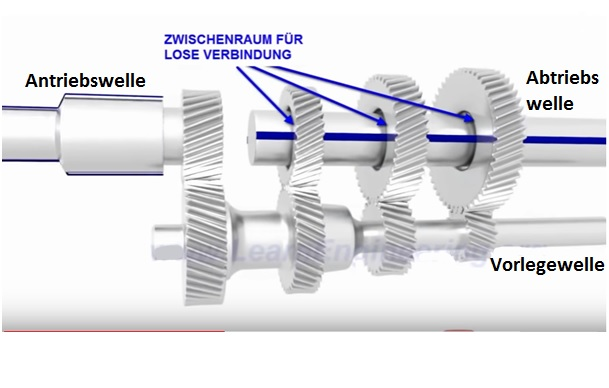
\includegraphics{Bilder/Fahrzeuggetriebe.jpg}
	\caption{Fahrzeuggetriebe}
	\label{fig:Fahrzeuggetriebe}
\end{figure}

\subsection{Getriebe des Prüfstands}

Der Prüfstand besitzt zwei Gänge, in die über eine Schaltgabel geschaltet werden kann. Eine Bewegung der Schaltgabel nach links legt Gang 1 über eine mechanische Synchronisierung ein, während mit Hilfe einer Bewegung nach rechts die Schaltung des Ganges 2 durch eine Klauenkupplung erfolgt. Somit können sowohl Schaltaktoriksysteme mit als auch ohne Synchronring untersucht werden.
Die Bewegung der Schaltgabel wird durch einen Linearaktor ermöglicht, welcher von außen an das Item-Profil verschraubt ist. In diesem ist eine Tauchspule verbaut, die die benötigten Kräfte auf die Läuferstange aufbringt. Über eine starre Wellenkupplung sind Läuferstange und Schaltgabel miteinander verbunden, wodurch die Kräfte auf die Schaltgabel übertragen werden und Schaltvorgänge ermöglicht werden.

\subsection{Aktor}

Der in dem Prüfstand verbaute Tauchspulenaktor wurde von Oliver Hahn im Rahmen seiner Bachelorthesis entwickelt und konstruiert. Er übernimmt die Aufgabe, die Schaltgabel  über die Schaltstange translatorisch zu verschieben. Sein Querschnitt ist in folgender Abbildung schematisch dargestellt.

\begin{figure}[h]
	\centering
		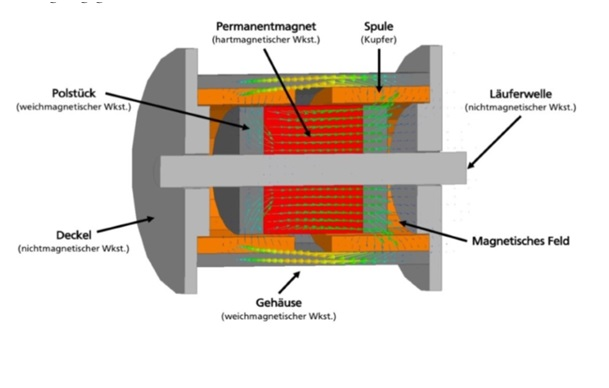
\includegraphics{Bilder/Querschnitt Aktor.jpg}
	\caption{Querschnitt Tauchspulenaktor}
	\label{fig:Querschnitt Aktor}
\end{figure}

Sein Aufbau ist zylindrisch und kann in den ortsfesten Stator und den beweglichen Läufer unterteilt werden. Der Stator des Aktors besteht aus zwei in Reihe geschalteten Kupferspulen, welche fest in dem Gehäuse aus Weicheisen liegen und nach oben und unten mit Deckeln aus Aluminium fixiert werden. Der Läufer besteht aus einer nichtmagnetischen Läuferwelle, auf der sich fünf Permanentmagneten aus Neodym-Eisen-Bor befinden, welche mit Hilfe von zwei Polstücken aus Weicheisen axial auf der Läuferstange montiert sind. 
Werden nun die Kupferspulen von Strom durchflossen, so wirkt eine vom Magnetfeld der Permanentmagneten induzierte Lorentzkraft orthogonal auf sie. Diese Kraft ist abhängig von der Stromstärke I, der magnetischen Flussdichte der Permanentmagneten B und der vom Magnetfeld durchsetzten Leiterlänge l:
	\[F=I*l*B
\]



%%%%%%%%%%%%%%%%%%%%%%%%%%%%%%%%%%%%%%%%%%

\listoffigures\addcontentsline{toc}{chapter}{\listfigurename}
\end{document}
